\documentclass[12pt,a4paper,twoside]{article}
\usepackage{amsmath}
\usepackage{physics}
\usepackage{amssymb}
\usepackage{graphicx}
\begin{document}

\subsubsection*{Identifiying importance sampling functions for Dual Scattering Approximation}
When doing importance sampling, we like to sample an incident direction $\omega_i$ given an outgoing direction $\omega_o$. The idea is to put more emphasis on samples that are important to the rendering equation than on samples that have a small effect.

Finding importance sampling functions for the dual scattering approximation requires finding functions in the rendering equation from which we can easily create a sample function.
To sample, we must obtain a pdf that is similar in shape to the rendering equation. Then this pdf must be integrated to a CDF and consequently this CDF must be inversed to be able to sample a direction vector, given a canonical random variable $\xi \in [0, 1]$.

The dual scattering algorithm can be defined as:

\begin{equation}
f(\omega_i, \omega_r) = 1
\end{equation}

The following functions can be identified from which we could draw samples.

According to~\cite{companion} 

\subsubsection*{Importance sampling the Marschner $N_{TT}$ equation}

The Marschner model consists of a seperation of longitudinal scatterig and azimuthal scattering. can be importance sampled using s simplification described in~\cite{sadeghi:10} 

\begin{equation}
N_{TT}(\phi) = g(\beta_{TT}, \pi - \phi)
\end{equation}

The gaussian function cannot be analytically integrated and inverted~\cite{pixarmemo}. To generate samples we need to resort to compute the inverse error function or numerical inversion~\cite{pixarmemo}. Another option is to make use of the Box-Muller tranform. The Box-Muller transform takes two uniformly distributed samples in the interval [0, 1] and maps them to two standard normally distributed samples~\cite{box-muller}.

\begin{eqnarray}
X = \sqrt{-2 \ln u_1} \cos 2\pi u_2 \\
Y = \sqrt{-2 \ln u_1} \sin 2\pi u_2 
\end{eqnarray}

Now that we are able to sample $\phi$ according to the gaussian distribution, there are still a few things that we must consider. First of all, the samples generated using this method are unbounded, which means that we can end up with values that are outside the range for $\phi \in [\-\pi, \pi]$. A way to solve this is to clamp the values to this range. Since this can lead to a bias in the sampling process, the likelihood of sampling outside of the range is very small and hardly noticable in the renderings~\cite{pixarmemo}.

\begin{align}
\phi & = \beta_{TT} \cdot \sqrt{-2 \ln u_1} \cos 2\pi u_2) & \textnormal{with $u_1, u_2 \in [0, 1]$}  \\
\phi_i & = \phi_r - (\pi - \phi) &&
\end{align}


Take into account that $\phi_i$ in itself must be wrapped properly to stay inside it's range as well.

Since we are sampling from a normalized gaussian function, we already have the pdf. Filling in the width $\beta_{TT}$ the pdf looks like.

\begin{equation}
pdf(\phi) = \frac{1}{\beta_{TT} \sqrt{2\pi}} \cdot e^{-\frac{1}{2}(\frac{\phi}{\beta_{TT}})^2}
\end{equation}

\subsubsection*{Importance sampling the longitudinal equations from Marschner $M_R$ equation}

The longitudinal functions for the Marschner model all follow the same shape. They are described by a Gaussian distribution, with each component $X \in \{R, TT, TRT\}$ having specific configurations for the width of the gaussian $\beta_X$ and the longitudinal shift $\alpha_X$ of the peak due to the hair strands being covered by tilted cuticle scales.

\begin{equation}
M_X = g(\beta_X, \theta_h - \alpha_X)
\end{equation}

As described in section~\ref{a} we can use the Box-Muller transform to sample from a Gaussian distribution. The idea is to first sample from the gaussian distribution and then adjust the value to incorporate the effects of the width and shift of the scattering lobes. Since the Gaussian distribution can lead to samples outside the allowed range, we have to make sure to clamp $\theta_h$ values below a certain maximum $\theta_{max}$ that depends on $\theta_r$ and the shift of the lobe $\alpha_X$. The sampled incident longitudinal angle can now easily be computed as $\theta_i = 2\theta_h - \theta_r$.

\begin{align}
\theta_{max} & = \frac{\pi}{2} - \left| \frac{\theta_r}{2} - \alpha_X\right| \\
\theta & = \beta_{X} \cdot \sqrt{-2 \ln u_1} \cos 2\pi u_2) & \textnormal{with $u_1, u_2 \in [0, 1]$}  \\
\theta_h & = \theta + \alpha_X & \textnormal{with $\left|\theta\right| \leq \theta_{max}$}\\
\theta_i & = 2 \theta_h - \theta &&
\end{align}

Since we are using a normalized Gaussian distribution to sample from, we immediately have the pdf. By filling in the scattering lobe width and shift, we end up with the following pdf.

\begin{equation}
pdf(\theta) = \frac{1}{\beta_{X} \sqrt{2\pi}} \cdot e^{-\frac{1}{2}(\frac{\theta}{\beta_{X}})^2}
\end{equation}

\subsubsection*{Importance sampling the Marschner azimuthal equations $N_R$ and $N_{TRT}$ from Marschner}

The Marschner azimuthal angles can be simplified by depending only on $\phi$ angles~\cite{sadeghi:10}. This simplification helps enormously to find a sampling function from the distributions.

\begin{align}
N_R = N_{TT} = \cos \frac{\phi}{2}
\end{align}

To sample from this distribution, we must perform some standard integrations to find the normalized probability density function. Then we can integrate the pdf to end up with a cumulative distribution function and subsequently inverse the function to have the inverse CDF to be able to sample from.

To find a probability density function $p(\phi)$ we must find a normalization factor $c$ such that the integral for $N_{R, TRT}$ from $\phi \in [-\pi, \pi]$ integrates to one. This derivation process is rather straightforward.

\begin{equation}
\int_{-\pi}^{\pi} p(\phi) \dd{\phi} = c \cdot \int_{-\pi}^{\pi} \cos \frac{\phi}{2} \dd{\phi} = 1
\end{equation}

To find the normalization factor we integrate over $\phi$.

\begin{align}
\frac{1}{c} & = \int_{-\pi}^{\pi} \cos \frac{\phi}{2} \dd{\phi} \\
 & = 2 \cdot \int_{-\frac{\pi}{2}}^\frac{\pi}{2} \cos u \dd{u}  & \textnormal{where  $u = \frac{\phi}{2}$}\\
 & = 2 \cdot \left[ \sin \frac{\phi}{2} \right]_{-\pi}^{\pi} = 2 \cdot (\sin \frac{\pi}{2} - \sin \frac{-\pi}{2}) = 4
\end{align}

The resulting normalization factor is $c = \frac{1}{4}$ which is used to normalize the probability density function. The cumulative distribution function $P$ follows similarly from the integral derivation we have just performed.

\begin{equation}
p(\phi) = \frac{ \cos \frac{\phi}{2}}{4} \cdot
\end{equation}

 \begin{align*}
P(\phi) & = \int_{-\pi}^{\phi} p(\phi') \dd{\phi'} = \int_{-\pi}^{\phi} \cos \frac{\phi'}{2} \dd{\phi'} \\
&  = 2 \cdot \left[\sin \frac{\phi'}{2} \right]_{-\pi}^{\phi} = 2 \cdot \left(\sin \frac{\phi}{2} + 1\right) \\
\end{align*}

The CDF maps the sample to the cumulative distribution probability, which starts at 0 and goes to 1. What we need is the inverse of the CDF to map from a cumulative probability value to a sample value. To be able to do this we need to invert the CDF to obtain the inverse cumulative distribution function. The inverse cumulative distribution function $P^{-1}(\xi)$ takes a canonical random uniform variable $\xi \in [0, 1]$, which maps back to a sample value $\phi$. Inversion is not so difficult and is show in equation~\ref{inverse_Nr}.

\begin{equation}
\phi = P^{-1}(\xi) = 2 \cdot \sin^{-1} \left( \frac{\xi}{2} - 1\right)
\end{equation}

\subsubsection*{Transmittance function}
\begin{equation}
T_f(n, \omega_i) = d_f \cdot \prod_{k=1}^{n} a_f(\theta_d) = d_f \cdot a_f(\theta_d)^n
\end{equation}
The transmittance function $T_f$ is not a pure material description that depends on incoming and outgoing directions. It also depends on the number of scatter events $n$ found along the incident lighting direction $\omega_i$. We do not know $\omega_i$, because this is the direction we are trying to sample in the first place.

In figure~\ref{fig:average_ab_af} you can see the amount of average forward scattered light for different $\theta_d$. It is shown for nonabsorbing hair, blonde hair and brown hair for different scatter counts.

\begin{figure}
  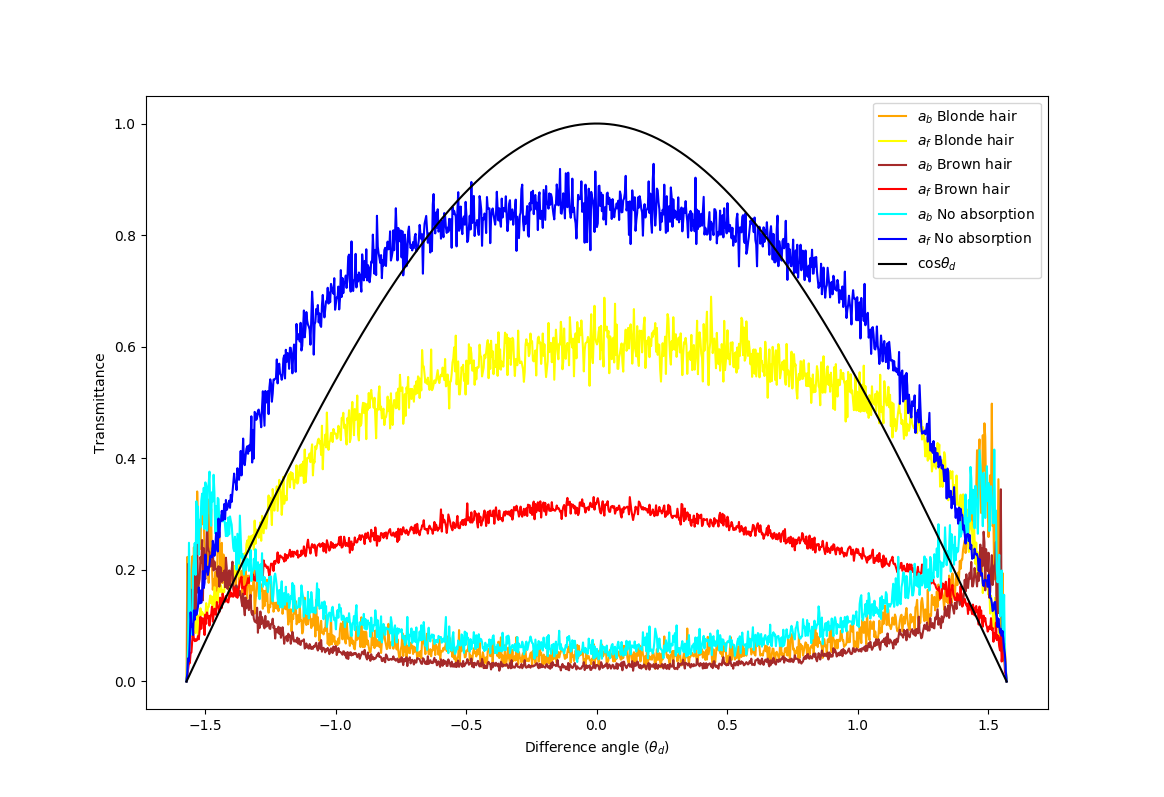
\includegraphics[width=\linewidth]{average_forward_backward_scattering_attenuation.png}
  \caption{Showing the average forward and backward transmittance. Nonabsorbing hair forward transmits a lot more light compared with colored hair. Also it can be seen that as the difference angle comes closer to +/-90 degrees, more light gets reflected back in the back hemisphere.}
  \label{fig:average_ab_af}
\end{figure}

By plotting the response for different scattering counts, we see that the scatter count only mutes the response. It has no real impact on the shape of the response graph, so we can create a pdf irrespective of the scatter count.


\begin{align*}
M_X & = g(\beta_X^2, \theta_h - \alpha_X) \\
N_R & = \cos\frac{\phi}{2} \\
N_{TT} & = g(\gamma_{TT}^2, \pi - \phi) \\
N_{TRT} & = \cos\frac{\phi}{2} \\
M_R^G & = g
\end{align*}


\subsubsection{Deriving pdf for $N_G$}

\begin{equation}
\begin{split}
N_R^G(\theta) & = \frac{1}{\pi} \cdot \int_{-\frac{\pi}{2}}^{\frac{\pi}{2}} \cos \frac{\phi'}{2} \dd{\phi'} \\
 & = \frac{2}{\pi} \int \cos u \dd{u}  = \frac{2}{\pi} \cdot \sin u \\
 & = \frac{2}{\pi} \cdot \left[\sin \frac{\phi}{2}\right]_{-\frac{\pi}{2}}^{\frac{\pi}{2}} = \frac{4}{\pi}
\end{split}
\end{equation}

It turns out that $N_R^G$ is dependent only on $\phi$, but in such a matter that $\phi$ is only relevant for front scattered radiance. To sample a $\phi$ we can just uniformly sample from the front hemisphere, giving the following PDF.

\begin{equation}
pdf[ N_R^G ](\phi) = \frac{1}{\pi}
\end{equation}


\bibliographystyle{ieeetr}
\bibliography{dualscattering_mis} 
\end{document}